\documentclass[
  man,
  longtable,
  nolmodern,
  notxfonts,
  notimes,
  colorlinks=true,linkcolor=blue,citecolor=blue,urlcolor=blue]{apa7}

\usepackage{amsmath}
\usepackage{amssymb}




\RequirePackage{longtable}
\RequirePackage{threeparttablex}

\makeatletter
\renewcommand{\paragraph}{\@startsection{paragraph}{4}{\parindent}%
	{0\baselineskip \@plus 0.2ex \@minus 0.2ex}%
	{-.5em}%
	{\normalfont\normalsize\bfseries\typesectitle}}

\renewcommand{\subparagraph}[1]{\@startsection{subparagraph}{5}{0.5em}%
	{0\baselineskip \@plus 0.2ex \@minus 0.2ex}%
	{-\z@\relax}%
	{\normalfont\normalsize\bfseries\itshape\hspace{\parindent}{#1}\textit{\addperi}}{\relax}}
\makeatother




\usepackage{longtable, booktabs, multirow, multicol, colortbl, hhline, caption, array, float, xpatch}
\setcounter{topnumber}{2}
\setcounter{bottomnumber}{2}
\setcounter{totalnumber}{4}
\renewcommand{\topfraction}{0.85}
\renewcommand{\bottomfraction}{0.85}
\renewcommand{\textfraction}{0.15}
\renewcommand{\floatpagefraction}{0.7}

\usepackage{tcolorbox}
\tcbuselibrary{listings,theorems, breakable, skins}
\usepackage{fontawesome5}

\definecolor{quarto-callout-color}{HTML}{909090}
\definecolor{quarto-callout-note-color}{HTML}{0758E5}
\definecolor{quarto-callout-important-color}{HTML}{CC1914}
\definecolor{quarto-callout-warning-color}{HTML}{EB9113}
\definecolor{quarto-callout-tip-color}{HTML}{00A047}
\definecolor{quarto-callout-caution-color}{HTML}{FC5300}
\definecolor{quarto-callout-color-frame}{HTML}{ACACAC}
\definecolor{quarto-callout-note-color-frame}{HTML}{4582EC}
\definecolor{quarto-callout-important-color-frame}{HTML}{D9534F}
\definecolor{quarto-callout-warning-color-frame}{HTML}{F0AD4E}
\definecolor{quarto-callout-tip-color-frame}{HTML}{02B875}
\definecolor{quarto-callout-caution-color-frame}{HTML}{FD7E14}

%\newlength\Oldarrayrulewidth
%\newlength\Oldtabcolsep


\usepackage{hyperref}




\providecommand{\tightlist}{%
  \setlength{\itemsep}{0pt}\setlength{\parskip}{0pt}}
\usepackage{longtable,booktabs,array}
\usepackage{calc} % for calculating minipage widths
% Correct order of tables after \paragraph or \subparagraph
\usepackage{etoolbox}
\makeatletter
\patchcmd\longtable{\par}{\if@noskipsec\mbox{}\fi\par}{}{}
\makeatother
% Allow footnotes in longtable head/foot
\IfFileExists{footnotehyper.sty}{\usepackage{footnotehyper}}{\usepackage{footnote}}
\makesavenoteenv{longtable}

\usepackage{graphicx}
\makeatletter
\def\maxwidth{\ifdim\Gin@nat@width>\linewidth\linewidth\else\Gin@nat@width\fi}
\def\maxheight{\ifdim\Gin@nat@height>\textheight\textheight\else\Gin@nat@height\fi}
\makeatother
% Scale images if necessary, so that they will not overflow the page
% margins by default, and it is still possible to overwrite the defaults
% using explicit options in \includegraphics[width, height, ...]{}
\setkeys{Gin}{width=\maxwidth,height=\maxheight,keepaspectratio}
% Set default figure placement to htbp
\makeatletter
\def\fps@figure{htbp}
\makeatother


% definitions for citeproc citations
\NewDocumentCommand\citeproctext{}{}
\NewDocumentCommand\citeproc{mm}{%
  \begingroup\def\citeproctext{#2}\cite{#1}\endgroup}
\makeatletter
 % allow citations to break across lines
 \let\@cite@ofmt\@firstofone
 % avoid brackets around text for \cite:
 \def\@biblabel#1{}
 \def\@cite#1#2{{#1\if@tempswa , #2\fi}}
\makeatother
\newlength{\cslhangindent}
\setlength{\cslhangindent}{1.5em}
\newlength{\csllabelwidth}
\setlength{\csllabelwidth}{3em}
\newenvironment{CSLReferences}[2] % #1 hanging-indent, #2 entry-spacing
 {\begin{list}{}{%
  \setlength{\itemindent}{0pt}
  \setlength{\leftmargin}{0pt}
  \setlength{\parsep}{0pt}
  % turn on hanging indent if param 1 is 1
  \ifodd #1
   \setlength{\leftmargin}{\cslhangindent}
   \setlength{\itemindent}{-1\cslhangindent}
  \fi
  % set entry spacing
  \setlength{\itemsep}{#2\baselineskip}}}
 {\end{list}}
\usepackage{calc}
\newcommand{\CSLBlock}[1]{\hfill\break\parbox[t]{\linewidth}{\strut\ignorespaces#1\strut}}
\newcommand{\CSLLeftMargin}[1]{\parbox[t]{\csllabelwidth}{\strut#1\strut}}
\newcommand{\CSLRightInline}[1]{\parbox[t]{\linewidth - \csllabelwidth}{\strut#1\strut}}
\newcommand{\CSLIndent}[1]{\hspace{\cslhangindent}#1}





\usepackage{newtx}

\defaultfontfeatures{Scale=MatchLowercase}
\defaultfontfeatures[\rmfamily]{Ligatures=TeX,Scale=1}





\title{A national longitudinal study of Muslim diversity and flourishing
in Aotearoa New Zealand: A quantitative study protocol}


\shorttitle{MDS - an NZAVS booster}


\usepackage{etoolbox}









\authorsnames[{1},{1},{2},{3},{1},{4},{5},{6},{1},{7},{1},{8},{1},{9},{10},{11},{1},{12},{1},{13},{14,15}]{Usman
Afzali,Jamila Badis,Parus Khoso,Gul e Aqsa,Farah Shawkat,Fatima
Junaid,Ayca Arkilic,Hussain Raissi,Hala Burhoum,Tuba Azeem,Iman
Husain,Zarqa Shaheen Ali,Zahra Haidary,Nasratullah Hamid,Zahra
Emamzadeh,Rizwan Sulehry,Somia Tasneem,Aarif Rasheed,Kumar
Yogeeswaran,Chris G. Sibley,Joseph A. Bulbulia}







\authorsaffiliations{
{School of Psychology, Speech and Hearing, University of
Canterbury},{College of Education, University of Canterbury},{School of
Health Sciences, University of Canterbury},{School of Management, Massey
University},{School of History, Philosophy, Political Science and
International Relations, Victoria University of Wellington},{School of
Social Science, University of Otago},{School of ABC, Victoria University
of Wellington},{ICL Business School, New Zealand Skills and Education
College},{School of Psychological Medicine, Universit of
Otago},{TBA, Ministry of Education},{School of Management, Victoria
University of Wellington},{Just Community},{School of
Psychology, University of Auckland},{School of Psychology, Victoria
University of Wellington},{Department of Linguistic and Cultural
Evolution, Max Planck Institute for Evolutionary Anthropology}}




\leftheader{Afzali, Badis, Khoso, Aqsa, Shawkat, Junaid, Arkilic, Raissi, Burhoum, Azeem, Husain, Ali, Haidary, Hamid, Emamzadeh, Sulehry, Tasneem, Rasheed, Yogeeswaran, Sibley and Bulbulia}



\abstract{The New Zealand Attitudes and Values Study is a longitudinal
study of social values and attitudes of New Zealanders that has started
in 2009 and collected data from thousands of subjects so far. Within the
realm of this study, negative attitudes towards minority groups, such as
discrimination and prejudice have been examined. Given that the Muslim
community has recently been subjected to a terrorist attack in
Christchurch, we decided to use data from the New Zealand Attitudes and
Values Study to look into Islamophobia from the Muslims' perspective, as
well as the remarkable resilience of Muslims despite many challenges. In
addition, we deemed necessary to investigate the overall wellbeing and
flourishing of Muslims, and whether values, identity, religiosity, and
meaning-making affect Muslims' self-perception and health outcomes.
However, we were limited by the sample size of Muslims within the New
Zealand Attitudes and Values Study to make such inferences. Therefore,
the current project was designed to boost the sample of Muslims within
the New Zealand Attitudes and Values Study over a three-year
quantitative longitudinal study. This protocol describes our pilot
community consultation, the decisions made and modified based on
consultation, community engagement, data collection, team, measures,
timeline, and proposed analyses, mostly focusing on the first year of
the booster. We also address the overall nuances in terms of perceived
enablers and challengers of data collection from a culturally distinct
minority religious community. We think that this protocol will be useful
to researchers who want to work with Muslims and similar communities in
New Zealand and globally.}

\keywords{Muslim, Islam, religion, diversity, discrimination, flourishing, meaning-making, identity}

\authornote{\par{\addORCIDlink{Usman
Afzali}{0000-0001-5119-9388}}\par{\addORCIDlink{Jamila
Badis}{0009-0005-2866-5033}}\par{\addORCIDlink{Parus
Khoso}{0000-0001-6384-038X}}\par{\addORCIDlink{Gul e
Aqsa}{0009-0003-0928-8039}}\par{\addORCIDlink{Farah
Shawkat}{0000-0000-0000-0001}}\par{\addORCIDlink{Fatima
Junaid}{0000-0002-6656-8120}}\par{\addORCIDlink{Ayca
Arkilic}{0000-0002-1775-3311}}\par{\addORCIDlink{Hussain
Raissi}{0000-0000-0000-0001}}\par{\addORCIDlink{Hala
Burhoum}{0000-0000-0000-0001}}\par{\addORCIDlink{Tuba
Azeem}{0000-0000-0000-0001}}\par{\addORCIDlink{Iman
Husain}{0000-0003-4032-4387}}\par{\addORCIDlink{Zarqa Shaheen
Ali}{0000-0002-7145-5788}}\par{\addORCIDlink{Zahra
Haidary}{0009-0000-5259-622X}}\par{\addORCIDlink{Nasratullah
Hamid}{0009-0002-0120-7428}}\par{\addORCIDlink{Zahra
Emamzadeh}{0009-0000-0000-0001}}\par{\addORCIDlink{Rizwan
Sulehry}{0000-0002-1209-0635}}\par{\addORCIDlink{Somia
Tasneem}{0000-0001-5471-6934}}\par{\addORCIDlink{Aarif
Rasheed}{0000-0000-0000-0001}}\par{\addORCIDlink{Kumar
Yogeeswaran}{0000-0002-1978-5077}}\par{\addORCIDlink{Chris G.
Sibley}{0000-0002-4064-8800}}\par{\addORCIDlink{Joseph A.
Bulbulia}{0000-0002-5861-2056}} 
\par{ }
\par{       }
\par{Correspondence concerning this article should be addressed to Usman
Afzali, School of Psychology, Speech and Hearing, University of
Canterbury, 20 Kirkwood Ave, Christchurch, Canterbury 8041, New
Zealand, Email: usman.afzali@canterbury.ac.nz}
}

\makeatletter
\let\endoldlt\endlongtable
\def\endlongtable{
\hline
\endoldlt
}
\makeatother
\RequirePackage{longtable}
\DeclareDelayedFloatFlavor{longtable}{table}

\urlstyle{same}



\makeatletter
\@ifpackageloaded{caption}{}{\usepackage{caption}}
\AtBeginDocument{%
\ifdefined\contentsname
  \renewcommand*\contentsname{Table of contents}
\else
  \newcommand\contentsname{Table of contents}
\fi
\ifdefined\listfigurename
  \renewcommand*\listfigurename{List of Figures}
\else
  \newcommand\listfigurename{List of Figures}
\fi
\ifdefined\listtablename
  \renewcommand*\listtablename{List of Tables}
\else
  \newcommand\listtablename{List of Tables}
\fi
\ifdefined\figurename
  \renewcommand*\figurename{Figure}
\else
  \newcommand\figurename{Figure}
\fi
\ifdefined\tablename
  \renewcommand*\tablename{Table}
\else
  \newcommand\tablename{Table}
\fi
}
\@ifpackageloaded{float}{}{\usepackage{float}}
\floatstyle{ruled}
\@ifundefined{c@chapter}{\newfloat{codelisting}{h}{lop}}{\newfloat{codelisting}{h}{lop}[chapter]}
\floatname{codelisting}{Listing}
\newcommand*\listoflistings{\listof{codelisting}{List of Listings}}
\makeatother
\makeatletter
\makeatother
\makeatletter
\@ifpackageloaded{caption}{}{\usepackage{caption}}
\@ifpackageloaded{subcaption}{}{\usepackage{subcaption}}
\makeatother

% From https://tex.stackexchange.com/a/645996/211326
%%% apa7 doesn't want to add appendix section titles in the toc
%%% let's make it do it
\makeatletter
\xpatchcmd{\appendix}
  {\par}
  {\addcontentsline{toc}{section}{\@currentlabelname}\par}
  {}{}
\makeatother

\begin{document}

\maketitle


\setcounter{secnumdepth}{-\maxdimen} % remove section numbering

\setlength\LTleft{0pt}


\section{Introduction}\label{sec-intro}

The devastating far-right extremist attack on two mosques in
Christchurch that killed 51 and injured another 49 Muslims
(\citeproc{ref-royalco2020}{\emph{Royal {C}ommission of {I}nquiry into
the Terrorist Attack on {C}hristchurch {M}asjidain on 15 {M}arch 2019},
2020}), albeit shocking to the world
(\citeproc{ref-worldle2019}{\emph{World Leaders Condemn New Zealand
Mosque Attacks}, 2019}) and unprecedented in New Zealand
(\citeproc{ref-jacinda2019b}{\emph{Jacinda {A}rdern on the
{C}hristchurch Shooting}, 2019}), was not as surprising to the Muslim
community and their leadreship (\citeproc{ref-rahman2019}{Rahman, 2019})
due to the widespread experience of Islamophobia and prejudice
(\citeproc{ref-sibley2020}{Sibley et al., 2020}). With oversease reports
showing increased Islamophobia following these attacks
(\citeproc{ref-islamoph2022}{\emph{Islamophobia After {C}hristchurch
Terror Attacks Quadrupled - {A}ustralian Report}, 2022}), we have
reasons to see an array of hope in New Zealand due to reports of recent
improved attitudes towards Muslims (\citeproc{ref-bulbulia2023}{Bulbulia
et al., 2023}; \citeproc{ref-shanaah2021}{Shanaah et al., 2021}). Most
of our research in this area, primarily from the New Zealand Attitudes
and Values Study (NZAVS) (\citeproc{ref-newzeal2024}{\emph{New Zealand
Attitudes and Values Study}, 2024}) lens, has so far shed light on such
attitudes from a non-Muslim perspective. In other words, we have
reported on how Muslims are perceived, and not how Muslims perceive
themselves. While the published NZAVS reports are an absolute necessity,
one can never underestimate the self-experience of Muslims themselves -
the direct victims of this heinous crime. This article aims to elaborate
on the protocol of a pioneering longitudinal study that is poised to
achieve the very goal -- examining Muslims' self-perception in New
Zealand from a variety of angles, as well as, the predictors of
resilience, flourishing, and wellbeing within Muslims. Given that the
Muslim community is positioned very uniquely in New Zealand: a minority,
historically stigmatized group that were direct victims of a terrorist
attacks and showed remarkable resilience (\citeproc{ref-anwar2020}{Anwar
\& Sumpter, 2020}; \citeproc{ref-royalco2020}{\emph{Royal {C}ommission
of {I}nquiry into the Terrorist Attack on {C}hristchurch {M}asjidain on
15 {M}arch 2019}, 2020}; \citeproc{ref-sibley2020}{Sibley et al.,
2020}), we had to consult with the community, make and/or amend
decisions based on the feedback received, and learn from other
stakeholders that had worked with community. Therefore, it is important
that such processes and decisions are recorded in the form of a study
protocol so that the future researchers in New Zealand and across the
globe can benefit and save valuable research time and resources.

\subsection{Perception of Muslims based on
NZAVS}\label{perception-of-muslims-based-on-nzavs}

The New Zealand Attitudes and Values Study (NZAVS) is a large
longitudinal national probability annual panel study of social
attitudes, personality, ideology and health outcomes that began in 2009
and has so far collected data from more than 70,000 subjects
(\citeproc{ref-newzeal2024}{\emph{New Zealand Attitudes and Values
Study}, 2024}). NZAVS has been instrumental in exploring minority
issues, including but not limited to discrimination, intergroup
relations, identity, distress, security, etc, and the dynamics and
mechanisms behind them. For instance, our findings indicated the
importance of national identity in Muslim perception
(\citeproc{ref-yogeeswaran2019}{Yogeeswaran et al., 2019}). More
specifically, the more one believed a specific ancestral heritage (being
European or Māori) or cultural aspects (ability to speak English) were
important for being considered a \emph{true} New Zealander, the lower
they rated their level of warmth toward Muslims
(\citeproc{ref-yogeeswaran2019}{Yogeeswaran et al., 2019}). A follow-up
longitudinal examination indicated that the warmth rating of Muslims has
historically been the lowest (based on data from 2012-2018) compared to
other minority groups (Indians, Chinese, immigrants in general, and
Asians in general), though, there was a small steady increase in warmth
towards all groups along these years (\citeproc{ref-sibley2020}{Sibley
et al., 2020}). Sibley et al. (\citeproc{ref-sibley2020}{2020}) also
indicated that lower education, lower socioeconomic status, being male,
older age, unemployment, lower agreeableness (based on Big-6 personality
test), and lower on openness (based on Big-6 personality test) predicted
lower warmth toward Muslims. Interestingly, but not unexpectedly, warmth
rating of Mulsims was increased unprecedentedly (above and beyond the
steady small increase reported in Sibley et al.
(\citeproc{ref-sibley2020}{2020})) following Christchurch shootings
(\citeproc{ref-shanaah2021}{Shanaah et al., 2021}), and sustained for
three years post shootings (\citeproc{ref-bulbulia2023}{Bulbulia et al.,
2023}). Bulbulia et al. (\citeproc{ref-bulbulia2023}{2023}) indicated
that shootings caused increase in warmth toward Muslims, but not toward
other groups -- known as negative controls -- stigmatised groups that
were not anticipated to be affected by the shootings (e.g., people with
mental illness, overweight people, and elderly people).

\textbf{Warmth vs islamophobia (Jamila).}

\textbf{Muslim political representation in the media (Ayca Arkilic).}

psychological effects.

\textbf{Perceived discrimination and belonging: Raissi}

This implied that has also explored perception of Muslims and the
mechanisms of attitudinal changes towards Muslims following 15 March
2019 Christchurch terrorist attacks (\citeproc{ref-byrne2022}{Byrne et
al., 2022}; \citeproc{ref-hawi2019}{Hawi et al., 2019};
\citeproc{ref-sibley2020}{Sibley et al., 2020};
\citeproc{ref-yogeeswaran2019}{Yogeeswaran et al., 2019}). However, much
of the NZAVS work to date with the Muslim community has focused on
conveying information about how Muslims are perceived. After receiving
strong positive signals from the Muslim community to scientifically
explore diversity, discrimination, self-perception, resilience,
meaning-making, and flourishing; this longitudinal study was conceived
to address such a worthwhile scientific need. This protocol addresses
our pilot community consultation, the decisions made and modified based
on consultation, community engagement, data collection, team, and
measures. The study primarily aims to explore the diveristy of Muslims
in New Zealand, assess Muslims' perceived discrimination in comparison
with other groups, unearth predictors of flourishing and meaning-making,
and measure the effect of service-attendance and
religious-identification on these constructs.

Introduce the context of the study, emphasizing the need to understand
the psychological impact of mass trauma events on diverse populations
such as the Christchurch Muslim community. Highlight the significance of
longitudinal research in assessing long-term mental health outcomes.

\begin{enumerate}
\def\labelenumi{\arabic{enumi}.}
\tightlist
\item
  Far right terrorism and attitudes toward Muslims (Usman)
\item
  Other research on Muslim wellbeing (Dr Fatima)
\item
  Other ongoing projects: Qual (Farah); and Islamophobia scale to verify
  our previous findings (Jamila).
\end{enumerate}

\section{Background}\label{background}

\begin{itemize}
\tightlist
\item
  Provide a brief overview of the Christchurch mosque attacks and their
  aftermath.
\item
  Discuss existing literature on the psychological effects of mass
  trauma events, particularly on diverse cultural groups.
\item
  Outline the gaps in current knowledge regarding the long-term
  psychological effects of such events on the Muslim community.
\end{itemize}

\section{Research Aims}\label{research-aims}

\begin{itemize}
\tightlist
\item
  Clearly state the research questions and objectives of the
  longitudinal study.
\item
  Emphasize the importance of assessing psychological outcomes over time
  to understand the trajectory of mental health in the affected
  population.
\end{itemize}

\subsection{Hypotheses}\label{hypotheses}

Given that the present project functions as a booster for NZAVS and uses
the same questionnaires, the questions that can be answered by MDS can
be limitless, and one coud suggest a large number of hypotheses to be
tested and questions that can be answered from these data in the years
to come. However, immediately we are trying to test the following
hypotheses -- within the span of MDS:

\emph{Hypothesis 1:} Muslims with the strongest ties to their community
as measured by service attendance and prayer are buffered most from
anti-Muslim prejudice.

\emph{Hypothesis 2:} Muslims experience greater challenges to employment
and health than matched members of other religious groups.

\emph{Hypothesis 3:} Subjective well-being, the meaning of life, and
psychological distress are similar among Muslims and matched members of
religious groups from the buffering of religious community-making.

Having sensed interest in these data from researchers in New Zealand and
overseas, it maybe possible to immediately test other hypotheses within
the realm of MDS, that would be published as independent research
articles.

\section{Method}\label{method}

\begin{itemize}
\item
  \textbf{Study Design:} Describe the longitudinal design of the study,
  including the planned follow-up periods.
\item
  \textbf{Participant Selection:} Define the inclusion criteria for
  participants, specifying age, residency, and other relevant factors.

  Mulsim = 1.3\% of New Zealand population.
\end{itemize}

\textbf{Materials}

NZAVS questionnaire has a large number of measures. Here, we are only
highlighting and explaining those that are pertinent to the readily
planned papers that are going to published from the booster study, with
levels of measurement indicated, as well as the reversed coded ones. For
Likert type scales, we are noting the the minimum and maximum level
along with description. For instance, \emph{(Not important 1-7 Very
important)} would mean that it is rated on a scale of 1 to 7 where 1
indicates not important and 7 indicates very important. Notwithstanding,
we might choose to report further measures too, which will then be
elaborated upon in the individual articles.

\begin{itemize}
\item
  Service attendance and religiosity:

  \begin{enumerate}
  \def\labelenumi{\arabic{enumi}.}
  \item
    Do you identify with a religion and/or spiritual group? (Yes/No). If
    yes, what religion or spiritual group? (String entry).
  \item
    How many times did you attend a church or place of worship in the
    last month? (String entry)
  \item
    How many times did you pray in the last week? (String entry)
  \item
    How many times did you read religious scripture in the last week?
    (String entry)
  \item
    How important is your religion to how you see yourself? (String
    entry) (Not important 1-7 Very important)
  \item
    I identify as a spiritual person. (Strongly Disagree 1-7 Strongly
    Agree)
  \item
    Do you believe in God? (Yes/No)
  \item
    Do you believe in any form of spirit or life force? (Yes/No)
  \end{enumerate}
\item
  Prejudice:

  \begin{enumerate}
  \def\labelenumi{\arabic{enumi}.}
  \item
    I feel that I am often discriminated against because of my
    religious/spiritual beliefs. (Strongly Disagree 1-7 Strongly Agree)
  \item
    People from my ethnic group are discriminated against in New
    Zealand. (Strongly Disagree 1-7 Strongly Agree)
  \item
    I feel that I am often discriminated against because of my age.
    (Strongly Disagree 1-7 Strongly Agree)
  \item
    I feel that I am often discriminated against because of my
    ethnicity. (Very Innacurate 1-7 Very Accurate)
  \item
    I feel that I am often discriminated against because of my gender.
    (Very Innacurate 1-7 Very Accurate)
  \end{enumerate}
\item
  Intergroup Warmth Ratings: Participants are asked to rate their
  feelings of warmth toward different groups using ``feeling thermometer
  scale'' for each group from least to most warmth on a 1-7 Likert scale
  (see Figure~\ref{fig-warmth} for reference). Groups include: NZ
  Europeans, Māori, Asians in general, Pacific Islanders, Elderly
  people, People with a disability, Refugees, Overweight people,
  Immigrants in general, Chinese, Indians, Muslims, LGBTQ+ people,
  People with mental illness.
\end{itemize}

\begin{figure}[!htbp]

{\caption{{Feeling thermometer scale}{\label{fig-warmth}}}}

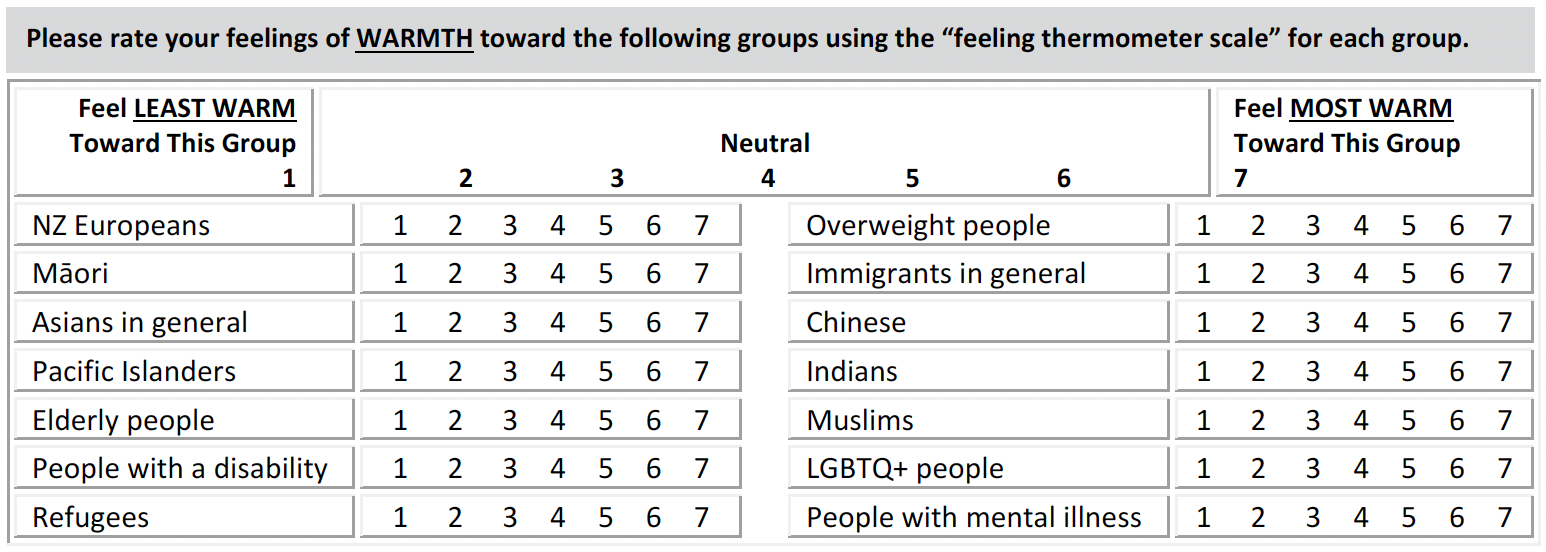
\includegraphics[width=0.75\textwidth,height=\textheight]{figs/warmth.png}

{\noindent \emph{Note.} From NZAVS Wave 15 \url{https://osf.io/75snb/}}

\end{figure}

\begin{itemize}
\item
  Felt belonging:

  \begin{enumerate}
  \def\labelenumi{\arabic{enumi}.}
  \item
    I know that people in my life accept and value me. (Very Innacurate
    1-7 Very Accurate)
  \item
    I feel like an outsider. (Very Innacurate 1-7 Very Accurate)
  \item
    I know that people in around me share my attitudes and beliefs.
    (Very Innacurate 1-7 Very Accurate)
  \end{enumerate}
\item
  Support:

  \begin{enumerate}
  \def\labelenumi{\arabic{enumi}.}
  \item
    There are people I can depend on to help me if I really need it.
    (Strongly Disagree 1-7 Strongly Agree)
  \item
    There is no one I can turn to for guidance in times of stress (R).
    (Strongly Disagree 1-7 Strongly Agree)
  \item
    I know there are people I can turn to when I need help. (Strongly
    Disagree 1-7 Strongly Agree)
  \end{enumerate}
\item
  Employment:

  \begin{enumerate}
  \def\labelenumi{\arabic{enumi}.}
  \item
    What is your highest level of qualification? (String entry)
  \item
    Are you currently employed (This includes self-employed of casual
    work)? (Yes/No). This leads to a four-point nominal response:
    employed full-time, employed part-time, unemployed, and not in the
    labour force.
  \item
    In that job, what is your current occupation (String entry)
  \item
    What is the main activity of the business or employer that you work
    for? (String entry)
  \item
    How long have you worked at your current organization? (String
    entry: years/months)
  \item
    How satisfied are you with your current job? (Not satisfied 1-7 Very
    satisfied)
  \item
    How secure do you feel in your current job? (Not secure 1-7 Very
    secure)
  \item
    How valued do you feel by your current organization? (Not valued 1-7
    Very valued)
  \end{enumerate}
\item
  Health:

  \begin{enumerate}
  \def\labelenumi{\arabic{enumi}.}
  \item
    In general, would you say your health is\ldots{} (Poor 1-7
    Excellent)
  \item
    I seem to get sick a little easier than other people. (Strogly
    disagree 1-7 Strongly agree)
  \item
    I expect my health to get worse. (Strogly disagree 1-7 Strongly
    agree)
  \item
    Do you have a health condition or disability that limits you, and
    that has lasted for 6+ months? (Yes/No). If yes, please state:
    (String entry)
  \item
    How often do you have a drink containing alcohol? Measured using a 6
    point nominal scale (Never - I don't drink, Monthly or less, Up to 4
    times a month, Up to 3 times a week, 4 or more times a week, Don't
    know)
  \item
    Have you ever regularly smoked tobacco cigarettes? (Yes/No).
  \item
    Have you ever regularly used e-cigarettes? (Yes/No).
  \item
    Do you currently smoke tobacco cigarettes? (Yes/No).
  \item
    Do you currently vape or use e-cigarettes? (Yes/No).
  \item
    Access to and satisfaction with GP: Do you have a regular family
    doctor/GP? (Yes/No). (If yes) How satisfied are you with the service
    and care you receive from your family doctor/GP? (Not satisfied 1-7
    Very satisfied). Do you think your doctor/GP shares a similar
    cultural background to you? (Definitely no 1-7 Definitely yes). Does
    your doctor/GP respect your cultural background when you are
    discussing health issues with them? (Definitely no 1-7 Definitely
    yes).
  \item
    Please estimate how many hours you spent during each of the
    following things last week (String entry). Options provided: Working
    in paid employment, housework/cooking, looking after children,
    volunteer/charitable work, exercising/physical activity, watching
    TV/Netflix/movies, travelling/commuting, watching/reading news,
    using the internet (in total), using social media (e.g., Facebook),
    playing video games/computer games.
  \item
    BMI: Calculated by using a person's weight (Kg) divided by square
    root of height (m) that are asked separately, using ``What is your
    height? (String entry (meters))'', and ``What is your weight?
    (String entry (kgs))''
  \item
    Forgiveness vs vengeful rumination: Sometimes I can't sleep because
    of thinking about past wrongs I have suffered., I can usually
    forgive and forget when someone does me wrong., I find myself
    regularly thinking about past times that I have been wronged. (1 =
    Strongly disagree, 7 = Strongly agree)
  \item
    During the past month, on average, how many hours of actual sleep
    did you get per night? (String entry)
  \item
    Do you have a health condition or disability that limits you, and
    that has lasted for 6+ months? (Yes/No). If yes, please state:
    (String entry)
  \item
    Chronic diseases diagnosis: See Figure~\ref{fig-chrondis}.
  \end{enumerate}
\end{itemize}

\begin{figure}[!htbp]

{\caption{{Chronic disease diagnosis}{\label{fig-chrondis}}}}

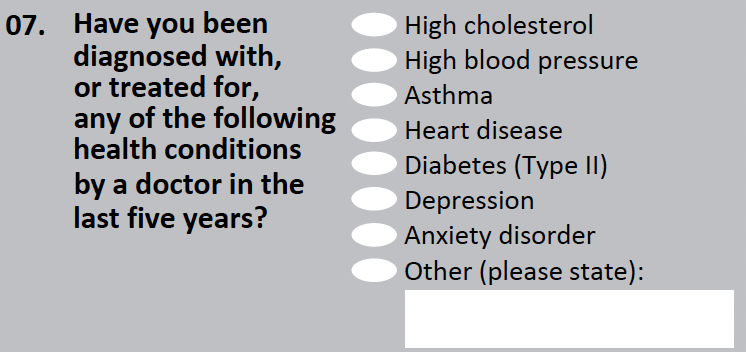
\includegraphics[width=0.75\textwidth,height=\textheight]{figs/chronic-disease.png}

{\noindent \emph{Note.} From NZAVS Wave 15 \url{https://osf.io/75snb/}}

\end{figure}

\begin{itemize}
\item
  Matching with other religious group: Similar to Bulbulia et al.
  (\citeproc{ref-bulbulia2023}{2023}), we will use the following
  demography and personality variables to identify matching members in
  different religions groups.

  \begin{enumerate}
  \def\labelenumi{\arabic{enumi}.}
  \item
    Age: What is your age? (String entry) and when is your date of birth
    (String entry)
  \item
    Education: An 11-point ordinal scale (No qualification 0-11 Doctoral
    degree, based on the New Zealand Qualification Framework
    (\citeproc{ref-thenew2016}{\emph{The New Zealand Qualifications
    Framework}, 2016})) based on the responses to the
    qualification-related question.
  \item
    Employment: A binary variable is created (0 = unemployed, 1 =
    employed) based on the responses to employment items ``Are you
    currently employed?''
  \item
    Ethnicity: The items displayed in Figure~\ref{fig-ethnicgroups} are
    categorised following the New Zealand Census Groups: European,
    Māori, Pacific Peoples, Asian, MELAA (Middle Eastern, Latin
    American/African), and Other.
  \item
    Gender: Responses to the string entry item ``What is your gender?'',
    gender will be used to create a binary measure (Male = 1, Not male =
    0).
  \item
    Socioeconomic status: Measured based on 2018 New Zealand Deprivation
    Index (\citeproc{ref-atkinson2019}{Atkinson et al., 2019}) that
    assigns a decile-rank index (Least deprived 1-10 Most deprived)
    using participants' immediate neighbourhood's aggregate census
    information. This index is calculated using component factor
    analysis of nine variables in weighted order as follows: proportion
    of adults who received a means-tested benefit, household income,
    proportion not owning own home, proportion of single-parent
    families, the proportion of unemployed, proportion lacking
    qualifications, proportion household crowding, proportion no
    telephone access, and proportion no car access. Hence, this index
    reflects nationwide mean deprivation level for small
    neighbourhood-type units (i.e., small community areas consisting
    about 80-90 people).
  \item
    Parent: Measured by assigning a binary variable (1 = those with
    children, 0 = the rest) to the item: How many children have you
    given birth to, fathered, or adopted? (String entry).
  \item
    Partner: Responses to ``What is you relationship status?'' are
    assigned a binary variable (1 = Has a partner, 0 = Doesn't have a
    partner).
  \item
    Religious identification: ``Yes'' responses to ``Do you identify
    with a religion and/or spiritual group?'' are assigned 1 and ``No''
    responses are coded 0.
  \item
    Political orientation: Based on responses to ``Please rate how
    politically left-wing versus right-wing you see yourself as being'',
    political orientation is assigned a 7-point scale (extremely
    left-wing 1-7 extremely right-wing).
  \item
    Residence: Urban or rural residence (a two-item nominal variable) is
    identified based on the physical addresses provided.
  \item
    Region of habituation (?)
  \item
    Occupational prestige (?)
  \item
    Race rejection anxiety:
  \item
    Big six personality traits: Six personality traits, agreeableness,
    conscientiousness, extraversion, openness, honesty-humility, and
    neuroticism, are measured using a 7-point (very inaccurate 1-7 very
    accurate) Mini-IPIP6 scale (\citeproc{ref-sibley2011}{Sibley et al.,
    2011}).
  \end{enumerate}
\end{itemize}

\begin{figure}[!htbp]

{\caption{{Ethnic Groups}{\label{fig-ethnicgroups}}}}

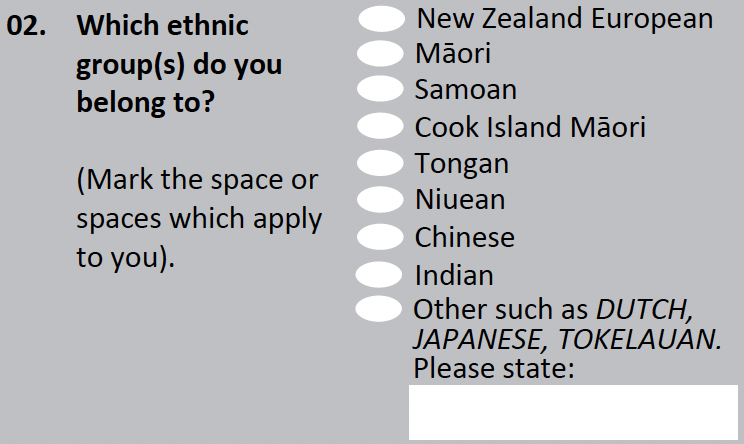
\includegraphics[width=0.75\textwidth,height=\textheight]{figs/ethnic-groups.png}

{\noindent \emph{Note.} From NZAVS Wave 15 \url{https://osf.io/75snb/}}

\end{figure}

\begin{itemize}
\tightlist
\item
  Subjective wellbeing/psychological distress: Measured using the
  Kessler-6 items (items 1-6 in Figure~\ref{fig-Kess-6}) rated on a
  5-point scale (None of the time 0-4 All of the time)
  (\citeproc{ref-kessler2010}{Kessler et al., 2010}).
\end{itemize}

\begin{figure}[!htbp]

{\caption{{Kessler 6}{\label{fig-Kess-6}}}}

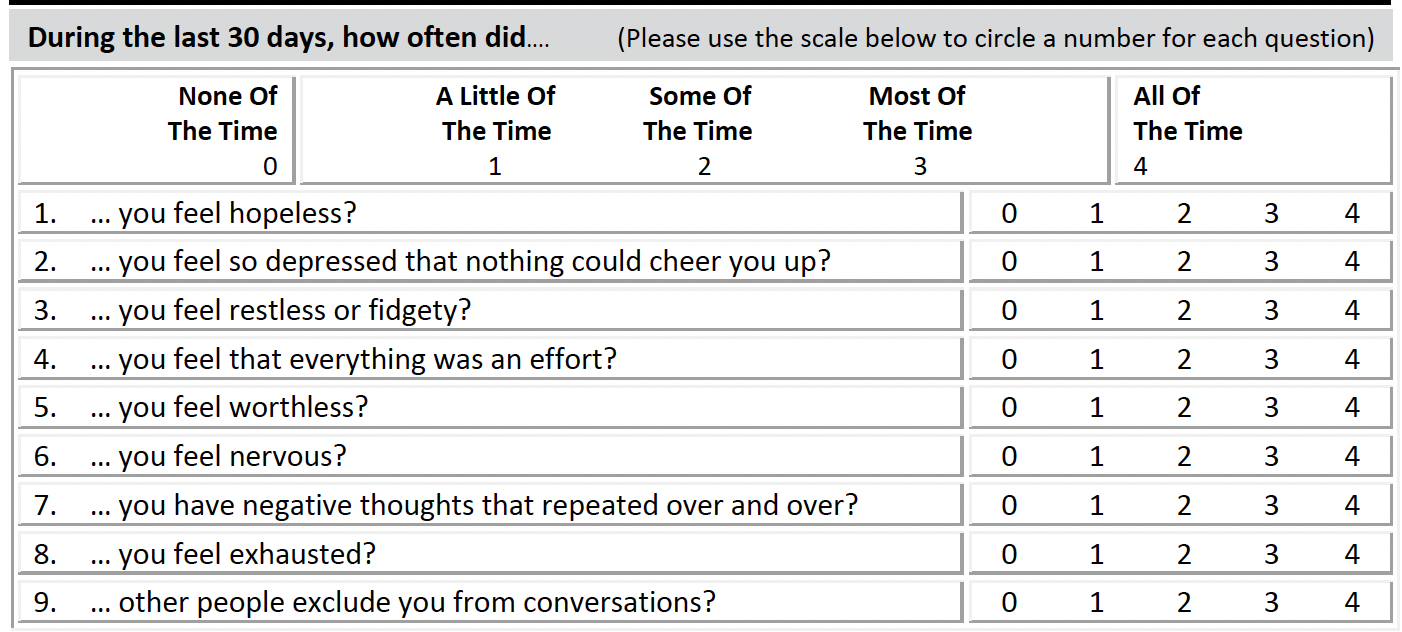
\includegraphics[width=0.75\textwidth,height=\textheight]{figs/kessler-6.png}

{\noindent \emph{Note.} From NZAVS Wave 15 \url{https://osf.io/75snb/}}

\end{figure}

\begin{itemize}
\item
  Meaning of life: My life has a clear sense of purpose (Strongly
  disagree 1-7 Strongly agree) and I have a good sense of what makes my
  life meaningful (Strongly disagree 1-7 Strongly agree).
\item
  Life satisfaction and national wellbeing: Items from
  Figure~\ref{fig-life-sat} measured on 11-item measure (Completely
  dissatisfied 0-10 Completely satisfied). In addition, ``I am satisfied
  with my life. (Strongly disagree 1-7 Strongly agree)'' and ``In most
  ways my life is close to ideal. (Strongly disagree 1-7 Strongly
  agree)''.
\end{itemize}

\begin{figure}[!htbp]

{\caption{{Life Satisfaction}{\label{fig-life-sat}}}}

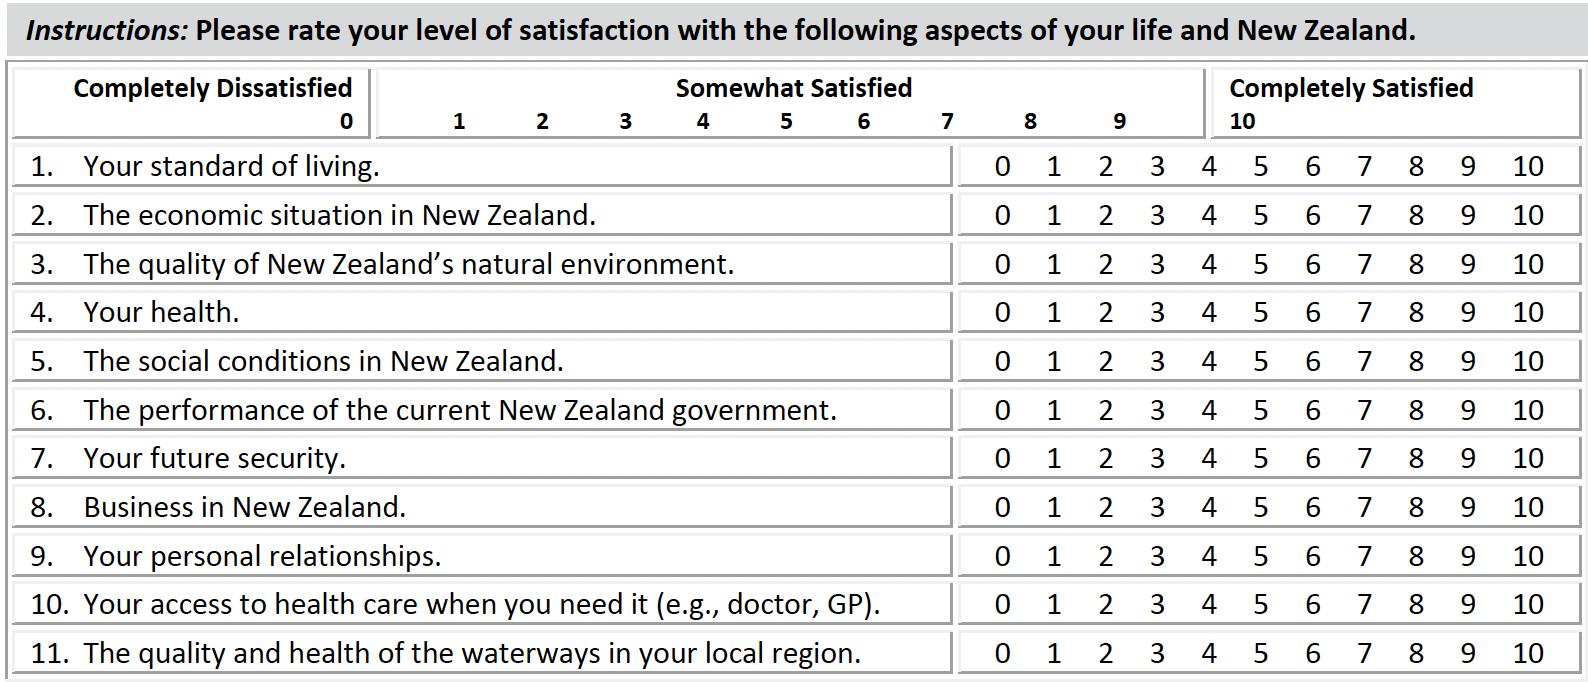
\includegraphics[width=0.75\textwidth,height=\textheight]{figs/life-sat.png}

{\noindent \emph{Note.} From NZAVS Wave 15 \url{https://osf.io/75snb/}}

\end{figure}

\begin{enumerate}
\def\labelenumi{\arabic{enumi}.}
\setcounter{enumi}{6}
\tightlist
\item
  Self esteem: On the whole am satisfied with myself. Take a positive
  attitude toward myself. Am inclined to feel that I am a failure.
\item
  Gratitude: I have much in my life to be thankful for. When I look at
  the world, I don't see much to be grateful for. I am grateful to a
  wide variety of people.
\item
  Community making: I feel a sense of community with others in my local
  neighbourhood (Strongly disagree 1-7 Strongly agree).
\item
  Values:
\item
  Resilience:
\end{enumerate}

\begin{itemize}
\item
  \textbf{Recruitment:} Detail the recruitment strategy, including
  outreach methods and sources of recruitment.
\item
  \textbf{Data Collection:} Explain the quantitative measures to be used
  in data collection, including validated self-report instruments and
  clinical assessments.
\end{itemize}

\begin{verbatim}
Warning: Using `size` aesthetic for lines was deprecated in ggplot2 3.4.0.
i Please use `linewidth` instead.
\end{verbatim}

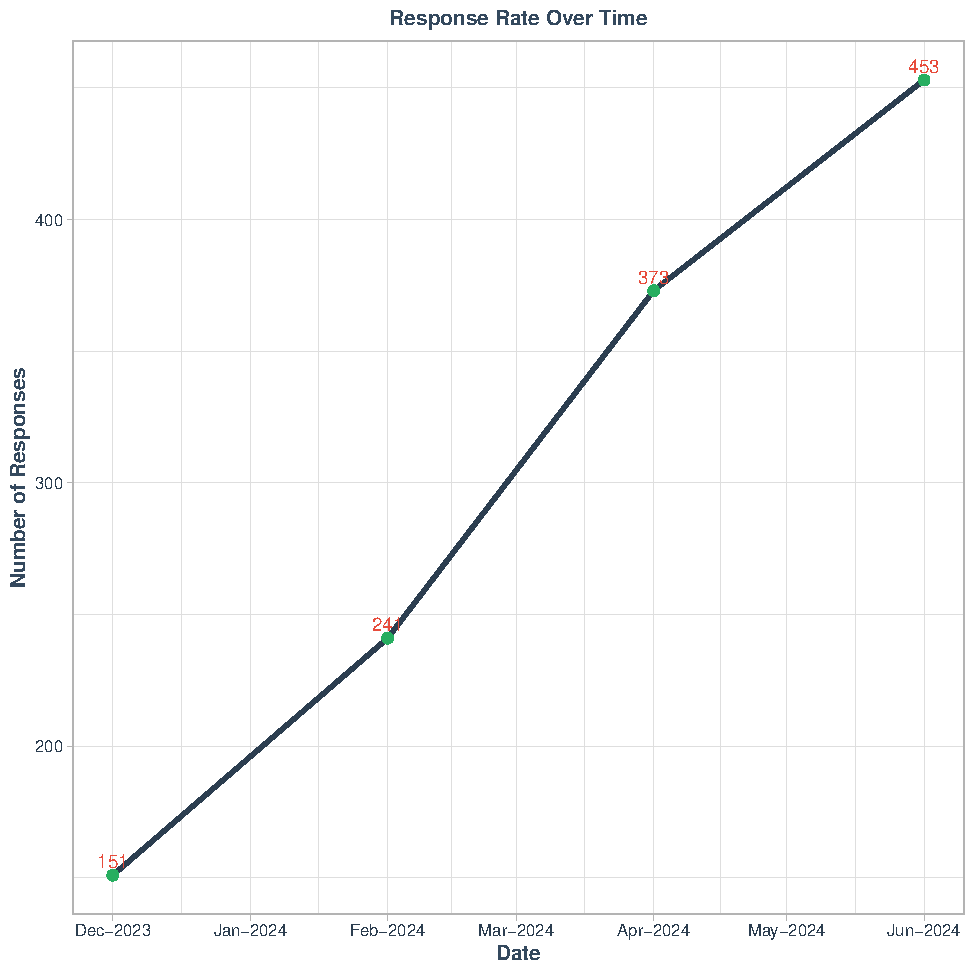
\includegraphics[width=0.5\textwidth,height=\textheight]{protocol_APA_files/figure-pdf/unnamed-chunk-6-1.pdf}

\begin{itemize}
\tightlist
\item
  \textbf{Procedure:} Outline the procedure for data collection at each
  time point, whether face-to-face or virtual.
\end{itemize}

\begin{enumerate}
\def\labelenumi{\arabic{enumi}.}
\tightlist
\item
  Community consultation in 2022: Aqsa and Parus
\item
  Current Wave general procedure: Usman and Jamila with input from all
  RA's: Farah, Hussain, Hala, Zarqa, Zahra H, Nasrat
\end{enumerate}

\begin{itemize}
\tightlist
\item
  \textbf{Ethical Considerations:} Discuss ethical approval obtained for
  the study and procedures for obtaining informed consent from
  participants.
\item
  \textbf{Data Analysis:} Provide an overview of the planned data
  analysis methods, including statistical techniques for longitudinal
  data analysis.
\item
  \textbf{Preregistration:} The design, hypotheses, measures, and
  anticipated data analysis are preregistered on OSF (). The study was
  preregistered before any attempted analyses of data.
\end{itemize}

\section{Expected Outcomes}\label{expected-outcomes}

\begin{itemize}
\tightlist
\item
  Anticipated findings based on the research questions and objectives.
\item
  Potential contributions of the study to the field of mental health
  research and implications for policy and practice.
\end{itemize}

\section{Timeline}\label{timeline}

\begin{itemize}
\tightlist
\item
  Present a timeline indicating key milestones in the study, including
  recruitment periods, data collection waves, and analysis phases.
\end{itemize}

\begin{enumerate}
\def\labelenumi{\arabic{enumi}.}
\tightlist
\item
  Usman and Jamila
\end{enumerate}

\begin{verbatim}
-- Attaching core tidyverse packages ------------------------ tidyverse 2.0.0 --
v dplyr     1.1.4     v readr     2.1.5
v forcats   1.0.0     v stringr   1.5.1
v lubridate 1.9.3     v tibble    3.2.1
v purrr     1.0.2     v tidyr     1.3.1
-- Conflicts ------------------------------------------ tidyverse_conflicts() --
x dplyr::filter() masks stats::filter()
x dplyr::lag()    masks stats::lag()
i Use the conflicted package (<http://conflicted.r-lib.org/>) to force all conflicts to become errors
\end{verbatim}

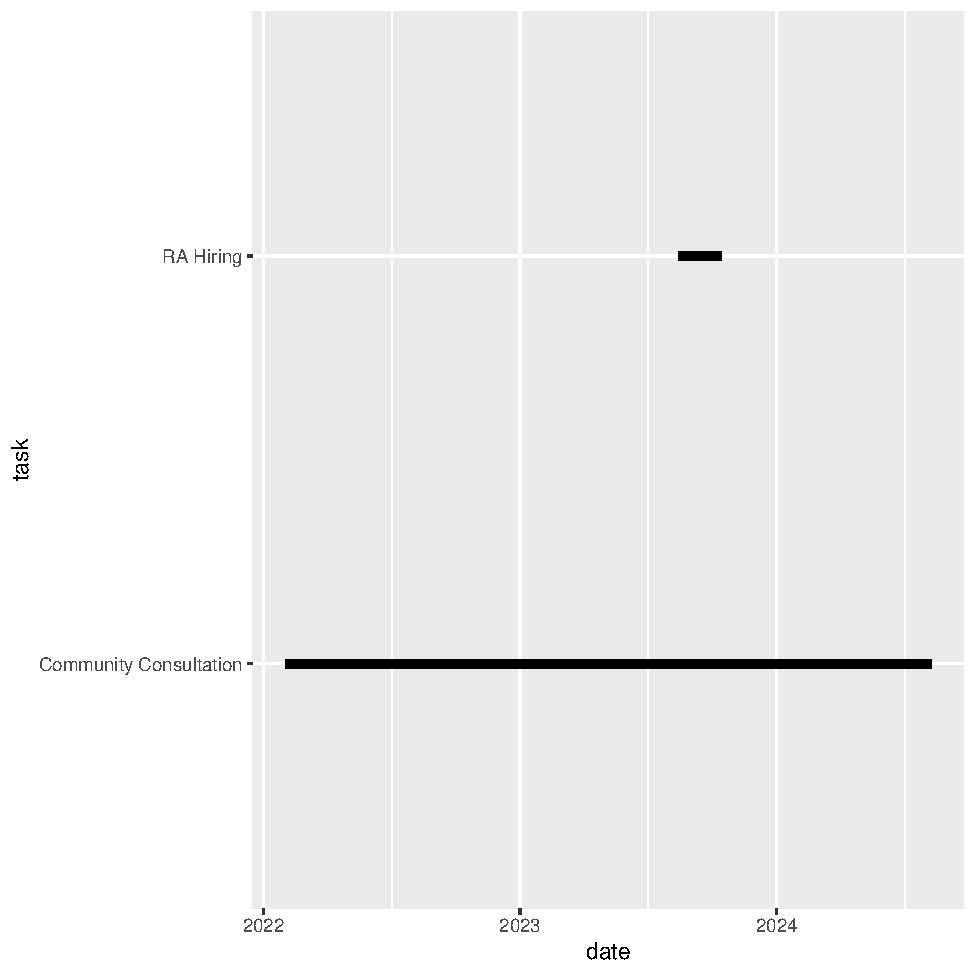
\includegraphics{protocol_APA_files/figure-pdf/unnamed-chunk-9-1.pdf}

\section{Strengths and Limitations}\label{strengths-and-limitations}

\begin{enumerate}
\def\labelenumi{\arabic{enumi}.}
\tightlist
\item
  Zahra E, Rizwan, Somia
\end{enumerate}

\section{Conclusion}\label{conclusion}

Summarize the importance of the longitudinal study in understanding the
psychological effects of the Christchurch mosque attacks on the Muslim
community and reiterate the significance of the research aims.

\begin{enumerate}
\def\labelenumi{\arabic{enumi}.}
\tightlist
\item
  Zahra E, Rizwan, Somia
\end{enumerate}

\section{Ethics}\label{ethics}

\section{Funding}\label{funding}

A National Longitudinal Study of Muslim Diversity and Flourishing
(famously knownas Muslim Diversity Study) is supported by a grant from
the Templeton Religion Trust(TRT-2022-30579). The funders had no role in
preparing the manuscript or the decisionto publish it.

\section{Data Availability}\label{data-availability}

The data described in this study are part of the Muslim Diversity Study,
that is conducted under the \href{https://osf.io/75snb/}{New Zealand
Attitudes and Values Study}.

\section{CoI}\label{coi}

We have no conflict of interest to disclose.

\newpage{}

\section{References}\label{references}

\phantomsection\label{refs}
\begin{CSLReferences}{1}{0}
\bibitem[\citeproctext]{ref-anwar2020}
Anwar, N. D., \& Sumpter, C. (2020). Societal resilience following
terrorism: community and coordination in Christchurch. \emph{Behavioral
Sciences of Terrorism and Political Aggression}, \emph{14}(1), 70--95.
\url{https://doi.org/10.1080/19434472.2020.1800785}

\bibitem[\citeproctext]{ref-atkinson2019}
Atkinson, J., Salmond, C., \& Crampton, P. (2019). \emph{NZDep2018 Index
of Deprivation}.

\bibitem[\citeproctext]{ref-bulbulia2023}
Bulbulia, J. A., Afzali, M. U., Yogeeswaran, K., \& Sibley, C. G.
(2023). Long-term causal effects of far-right terrorism in New Zealand.
\emph{PNAS Nexus}, \emph{2}(8).
\url{https://doi.org/10.1093/pnasnexus/pgad242}

\bibitem[\citeproctext]{ref-byrne2022}
Byrne, K. G., Yogeeswaran, K., Dorahy, M. J., Gale, J., Afzali, M. U.,
Bulbulia, J., \& Sibley, C. G. (2022). Psychological impact of far-right
terrorism against Muslim minorities on national distress, community, and
wellbeing. \emph{Scientific Reports}, \emph{12}(1), 1620.
\url{https://doi.org/10.1038/s41598-022-05678-x}

\bibitem[\citeproctext]{ref-hawi2019}
Hawi, D., Osborne, D., Bulbulia, J., \& Sibley, C. G. (2019). Terrorism
anxiety and attitudes toward muslims. \emph{New Zealand Journal of
Psychology (Online)}, \emph{48}(1), 8089.

\bibitem[\citeproctext]{ref-islamoph2022}
\emph{Islamophobia after {C}hristchurch terror attacks quadrupled -
{A}ustralian report}. (2022).
\url{https://www.rnz.co.nz/news/national/463304/islamophobia-after-christchurch-terror-attacks-quadrupled-australian-report}

\bibitem[\citeproctext]{ref-jacinda2019b}
\emph{Jacinda {A}rdern on the {C}hristchurch shooting: 'One of {N}ew
{Z}ealand's darkest days'}. (2019).
\url{https://www.theguardian.com/world/2019/mar/15/one-of-new-zealands-darkest-days-jacinda-ardern-responds-to-christchurch-shooting}

\bibitem[\citeproctext]{ref-kessler2010}
Kessler, R. C., Green, J. G., Gruber, M. J., Sampson, N. A., Bromet, E.,
Cuitan, M., Furukawa, T. A., Gureje, O., Hinkov, H., Hu, C.-Y., Lara,
C., Lee, S., Mneimneh, Z., Myer, L., Oakley-Browne, M., Posada-Villa,
J., Sagar, R., Viana, M. C., \& Zaslavsky, A. M. (2010). Screening for
serious mental illness in the general population with the K6 screening
scale: results from the WHO World Mental Health (WMH) survey initiative.
\emph{International Journal of Methods in Psychiatric Research},
\emph{19}(S1), 4--22. \url{https://doi.org/10.1002/mpr.310}

\bibitem[\citeproctext]{ref-newzeal2024}
\emph{New Zealand Attitudes and Values Study}. (2024).
\url{https://osf.io/75snb/}

\bibitem[\citeproctext]{ref-rahman2019}
Rahman, A. (2019). \emph{Islamic {W}omen's {C}ouncil repeatedly lobbied
to stem discrimination}.
\url{https://www.rnz.co.nz/news/on-the-inside/384911/islamic-women-s-council-repeatedly-lobbied-to-stem-discrimination}

\bibitem[\citeproctext]{ref-royalco2020}
\emph{Royal {C}ommission of {I}nquiry into the terrorist attack on
{C}hristchurch {M}asjidain on 15 {M}arch 2019}. (2020).
\url{https://christchurchattack.royalcommission.nz}

\bibitem[\citeproctext]{ref-shanaah2021}
Shanaah, S., Yogeeswaran, K., Greaves, L., Bulbulia, J. A., Osborne, D.,
Afzali, M. U., \& Sibley, C. G. (2021). Hate begets warmth? The impact
of an anti-{M}uslim terrorist attack on public attitudes toward
{M}uslims. \emph{Terrorism and Political Violence}, 119.

\bibitem[\citeproctext]{ref-sibley2020}
Sibley, C. G., Afzali, M. U., Satherley, N., Ejova, A., Stronge, S.,
Yogeeswaran, K., Grimshaw, M., Hawi, D., Mirnajafi, Z., \& Barlow, F. K.
(2020). Prejudice toward {M}uslims in {N}ew {Z}ealand: Insights from the
{N}ew {Z}ealand {A}ttitudes and {V}alues {S}tudy. \emph{New Zealand
Journal of Psychology}, \emph{49}(1).

\bibitem[\citeproctext]{ref-sibley2011}
Sibley, C. G., Luyten, N., Purnomo, M., Mobberley, A., Wootton, L. W.,
Hammond, M., Sengupta, N., Perry, R., West-Newman, T., Wilson, M.,
McLellan, L., Hoverd, W. J., \& Robertson, A. (2011). The mini-IPIP6:
Validation and extension of a short measure of the big-six factors of
personality in new zealand. \emph{New Zealand Journal of Psychology},
\emph{40}(3), 142--159.

\bibitem[\citeproctext]{ref-thenew2016}
\emph{The New Zealand Qualifications Framework}. (2016).

\bibitem[\citeproctext]{ref-worldle2019}
\emph{World leaders condemn New Zealand mosque attacks}. (2019).
\url{https://www.aljazeera.com/news/2019/3/15/the-world-reacts-to-new-zealand-mosque-attacks}

\bibitem[\citeproctext]{ref-yogeeswaran2019}
Yogeeswaran, K., Afzali, M. U., Andrews, N. P., Chivers, E. A., Wang,
M.-J., Devos, T., \& Sibley, C. G. (2019). Exploring new zealand
national identity and its importance for attitudes toward muslims and
support for diversity. \emph{New Zealand Journal of Psychology
(Online)}, \emph{48}(1), 29--35.

\end{CSLReferences}

\newpage{}

\section{Acknowledgements}\label{acknowledgements}

W. Joel Schneider for the
\href{https://github.com/wjschne/apaquarto}{Quarto template}.

\newpage{}

\section{CRediT Taxonomy Statement}\label{credit-taxonomy-statement}

\textbf{M. Usman Afzali:} Conceptualization, Methodology, Formal
analysis, Investigation, Resources, Data Curation, Writing - Original
Draft, Writing - Review \& Editing, Visualization, Supervision, Project
Administration, Funding Acquisition. \textbf{Jamila Badis:} Data
Curation, Project Administration, Writing - Original Draft, Writing -
Review \& Editing. \textbf{Parus Khoso:} Formal analysis, Data Curation,
Writing - Original Draft (Pilot Community Consultation), Writing -
Review \& Editing. \textbf{Gul e Aqsa:} Formal analysis, Data Curation,
Writing - Original Draft (Pilot Community Consultation), Writing -
Review \& Editing. \textbf{Farah Shawkat:} Data Curation, Writing -
Original Draft (Other Related Work), Writing - Review \& Editing.
\textbf{Fatima Junaid:} Writing - Original Draft (Introduction), Writing
- Review \& Editing. \textbf{Ayca Arkilic:} Writing - Original Draft
(Introduction), Writing - Review \& Editing. \textbf{Hussain Raissi:}
Writing - Original Draft (Method), Writing - Review \& Editing.
\textbf{Hala Burhoum:} Data Curation, Writing - Original Draft (Method),
Writing - Review \& Editing. \textbf{Tuba Azeem:} Data Curation, Writing
- Original Draft (Method), Writing - Review \& Editing. \textbf{Iman
Husain:} Data Curation, Writing - Original Draft (Method), Writing -
Review \& Editing. \textbf{Zarqa Shaheen Ali:} Data Curation, Writing -
Original Draft (Method), Writing - Review \& Editing. \textbf{Zahra
Haidary:} Data Curation, Writing - Original Draft (Method), Writing -
Review \& Editing. \textbf{Nasratullah Hamid:} Data Curation, Writing -
Original Draft (Method), Writing - Review \& Editing. \textbf{Zahra
Emamzadeh:} Writing - Original Draft (Strengths and Limitations,
Conclusion), Writing - Review \& Editing. \textbf{Rizwan Sulehry:}
Writing - Original Draft (Strengths and Limitations, Conclusion),
Writing - Review \& Editing. \textbf{Somia Tasneem:} Writing - Original
Draft (Strengths and Limitations, Conclusion), Writing - Review \&
Editing. \textbf{Aarif Rasheed:} Conceptualization, Data Curation,
Writing - Review \& Editing, Funding Acquisition. \textbf{Kumar
Yogeeswaran:} Conceptualization, Methodology, Writing - Original Draft,
Writing - Review \& Editing, Funding Acquisition. \textbf{Chris G.
Sibley:} Conceptualization, Methodology, Resources, Data Curation,
Supervision, Writing - Original Draft, Writing - Review \& Editing,
Project Administration, Funding Acquisition. \textbf{Joseph A.
Bulbulia:} Conceptualization, Methodology, Resources, Supervision,
Writing - Original Draft, Writing - Review \& Editing, Project
Administration, Funding Acquisition.

\appendix

\section{Title for Appendix}\label{title-for-appendix}






\end{document}
